\documentclass{article}
\usepackage{mathtools}
\usepackage{amssymb}
\usepackage{amsthm}
\usepackage{physics}
\usepackage{stmaryrd}
\usepackage{bbm}
\usepackage{hyperref}
\usepackage{tikz}
\usetikzlibrary{calc}
\usepackage{pgfplots}
\usepackage{minted}
\usepackage{subcaption}
\usepackage{graphicx}
\usepackage[margin=2cm]{geometry}
\hypersetup{
    colorlinks=true,
    linkcolor=blue,
    }
\usepackage{biblatex}
\addbibresource{refs.bib}
\usepackage{indentfirst}
\setlength{\parindent}{0.5cm}
\DeclareMathOperator{\Img}{Im}
\DeclareMathOperator{\Com}{Com}
\DeclareMathOperator{\End}{End}
\DeclareMathOperator{\Ker}{Ker}
\newtheorem{theorem}{Theoreme}
\newtheorem*{corollary}{Corollary}
\newtheorem{proposition}{Proposition}
\newtheorem{definition}{Definition}
\newtheorem{lemma}{Lemma}
\newtheorem{example}{Exemple}
\newtheorem{tactic}{Tactic}
\newcommand{\C}{\mathbb{C}}
\renewcommand{\L}{\mathcal{L}}
\newcommand{\Cn}{\mathscr{C}}
\renewcommand{\P}{\mathbb{P}}
\newcommand{\Z}{\mathbb{Z}}
\newcommand{\Q}{\mathbb{Q}}
\newcommand{\N}{\mathbb{N}}
\newcommand{\R}{\mathbb{R}}
\newcommand{\K}{\mathbb{K}}
\newcommand{\F}{\mathcal{F}}
\newcommand{\RM}[1]{\paragraph{RM} #1}
\DeclareMathOperator{\conv}{conv}

\begin{document}

\tableofcontents

\section{Motivation}

We were given several datasets from the website ??? which sells a variety of board games. This website collects data for every article, such as reviews and grades posted by the users. 

Our task was to treat and analyze this data to try to gain information from it. One purpose was to classify these reviews and being able to predict the sentiment of review (positive or negative). 

\section{Analysis on the data}

\subsection{Game score - comment}

\begin{figure}[h]
  \centering
  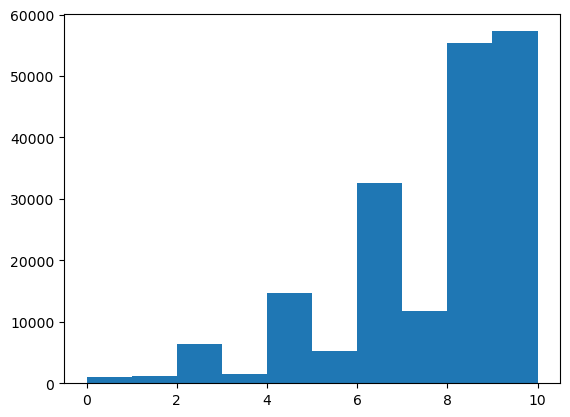
\includegraphics[height=4cm]{scores.png}
\end{figure}

\subsection{Game type - description}

\section{Corpus to vectors}

\subsection{Preprocessing}

Raw text data might contain unwanted or unimportant text due to which our results might not give efficient accuracy, and might make it hard to understand and analyze. So, proper pre-processing must be done on raw data.

We had to remove punctuation, URLs, numbers, accents, stopwords.
Stopwords are commonly used words in a language that are considered to have little or no significance in determining the meaning of a text.
`not' is not a stopword, because it might indicate the opposite sentiment.

We also applied Stemming that reduces words to their root forms. It minimizes the confusion around words that have similar meanings and lowers the complexity of the input space. However, it comes at the cost of throwing information away.

\subsection{One Hot Encoding}

One Hot Encoding is a vector representation of a word in vocabulary, ie the unique list of all the words appearing in the documents.
If the vocabulary size is n, each word in the vocabulary is therefore represented as a vector of size n. It takes binary values: 1 for the corresponding word and 0 otherwise.

\paragraph{On the implementation:}

We can represent the set of sentences as a tensor of shape (a, b, c) ie a matrices (number of sentences) of shape (b,c) where b represents the number of words in the sentence and c the vocabulary size.

\paragraph{Advantages:}

\begin{itemize}
  \item Intuitive and easy to implement
\end{itemize}

\paragraph{Inconvenients:}

\begin{itemize}
  \item Increase in dimensionality: a large vocabulary size implies a large number of columns, taking more memory size, which results in an increase in computational cost. + The matrix is sparse.
  \item Every vector sits in the orthogonal vector space so vectors are perpendicular to each other and are considered independent to each other, which is rarely the case.
  \item High chance of multi-collinearity due to dummy variables, which might affect the performance of the model (cf. Dummy Variable Trap)
\end{itemize}

\subsection{Bag of Words}

\subsection{tf-idf}

The BoW (Bag of Words) model assumes that the importance of a term is directly proportional to
the number of its appearance in the document, this can easily be misleading
when the most common words are `stopwords'. (But it really depends on
the algorithm that we are going to use afterwards, if we do perceptron, it wouldn't matter.)

But the BoW gives vectors with integer features, which may be favorable by some algorithm,
like Naive Bayes below. This being said, the tf-idf embedding gives vectors with features in $\mathbb{Q}$,
which can be dilated to integers.

tf-idf (term frequency - inverse document frequency) first considers
the whole of a corpus, it assumes a term too frequent in the corpus has little
information. Then it considers the importance of a term in a document
as the frequency of the term in this document times a scalar
representing its information in the corpus.

$$
\begin{aligned}
\mathrm{tfidf}(\mathrm{term}) & = \mathrm{tf}(\mathrm{term}) \times \mathrm{idf}(\mathrm{term}) \\
\mathrm{tf}(\mathrm{term}) & = \frac{\# \text { of times term appears in document }}{\# \text { of terms in document }} \\
\mathrm{idf}(\mathrm{term}) & =\ln \left(\frac{\# \text { of documents }}{\# \text { of documents in corpus with term }}\right)
\end{aligned}
$$

Other possible choices:

\begin{itemize}
  \item A term can be many (succesive) words (n-gram) (e.g. to
  take into account of negations before a word)
  \item The exact formulae can be changed while the same idea remains
\end{itemize}

\paragraph{On the implementation} Il faut éviter utiliser \verb|for|, et
utiliser les fonctions numpy à la place; on utilise les matrices sparse pour
gagner de la mémoire et parfois l'éfficacité.

\paragraph{Observations}
\begin{itemize}
  \item Curse of dimensionality
  \item Preprocessing is important
\end{itemize}

\section{Treating vectors}

\subsection{Protocol of the evaluation}

Can specify random seed to ensure reproductivity....

\subsection{Distances}

We can use euclidean distance, or we can use the distance concerning
only the angle between 2 vectors (so the `difference of lengths' of documents
is ignored).

$$
\begin{aligned}
&\text{(cosine similarity)}S(A, B) :=
\cos (\theta)=\frac{A \cdot B}{\|A\|\|B\|}\\
&\text{(cosine distance)}D(A, B) :=1-S(A, B)
\end{aligned}
$$

We see that cosine distance is better in nlp for 1. no curse of dimensionality; 2. no
need to reduce the dimension.

\subsection{Dimensionality reduction}

\begin{itemize}
  \item PCA (not useful for us, every new word (if not a stopword) can not be ignored and their linear combinations have no meaning)
  \item t-SNE (only useful for visulization?)
\end{itemize}

After the reduction of dimensionality, we may do a visulization; but
bad visulization results don't necessarily mean bad classification result.

\subsection{k nearest neighbour}

\paragraph{Algorithm} One predicts the information associated with a vector by the majority
of information associated with its neighbours (within k nearest).
We use tf-idf embedding here.
By simple experience
and raisonning (the length doesn't affect the positivity) as well, we chose cosine distance.

For comments of grades 4 - 7, they are more or less neutral, we can't
say if it is definitely positive or negative as human-being, so less chance
for our more or less naïve algorithm. For this reason we chose
to do our algorithm on comments of extremities.

To begin with, we delibrately balanced the data, 50\% of positive comments (5000)
and 50\% of negative comments (5000).

By adjusting the k, we obtained such result shown in Figure~\ref{fig:knn1}.

\begin{figure}[htbp]
  \centering
  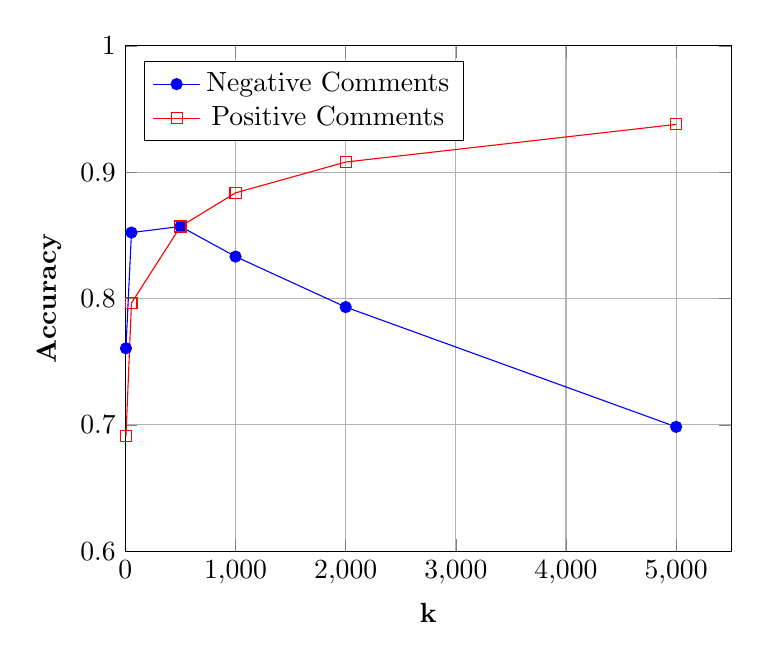
\begin{tikzpicture}
      \begin{axis}[
          xlabel={\textbf{k}},
          ylabel={\textbf{Accuracy}},
          xmin=0, xmax=5500,
          ymin=0.6, ymax=1,
          xtick={0,1000,2000,3000,4000,5000},
          ytick={0.6,0.7,0.8,0.9,1},
          legend pos=north west,
          grid=both,
          grid style={line width=0.2pt, draw=gray!30},
          major grid style={line width=0.4pt,draw=gray!60},
          height=8cm,
      ]
      \addplot[color=blue, mark=*] coordinates {
          (5,0.7606)
          (55,0.8522)
          (500,0.857)
          (1000,0.8332)
          (2000,0.7932)
          (5000,0.6984)
      };
      \addplot[color=red, mark=square] coordinates {
          (5,0.691)
          (55,0.7964)
          (500,0.857)
          (1000,0.8836)
          (2000,0.908)
          (5000,0.9378)
      };
      \legend{Negative Comments, Positive Comments}
      \end{axis}
  \end{tikzpicture}
  \caption{k nearest neighbor on balanced data}
  \label{fig:knn1}
\end{figure}

That was some good results. But in the reality, our data is extremely disporpotional,
if we apply knn directly, the algorithm would predict positive almost everytime. (Although
a positive comment has less chance to enter the neighbourhood of a negtive comment,
there are too many of them.) Indeed, we tried and get 0.26 as accuracy for negative comments and 0.94 for
positive comments.

The accuracy in total (on the data set) was good but it was not what we are after. We would like
$(r_p+r_n)/2$ to be big (so in the previous case it was 0.6). $r_{p/n}$ is the accuracy on the positive/negative comments.

To solve this problem, we add a parameter to our algorithm: \textbf{balance}.
balance is a float >= 1 meaning that we trim the list of data of one label
of more quantity to size = balance$\times$(number of data with another label).

As the Figure~\ref{fig:balancenk} shows, the balance value would
better stay at 1 (otherwise it damages significantly
the accuracy on the negatives) and we increase k to
remedy the disadvantage of positive prediction.

\begin{figure}[htbp]
  \centering
  \begin{subfigure}[t]{0.33\textwidth}
    \centering
    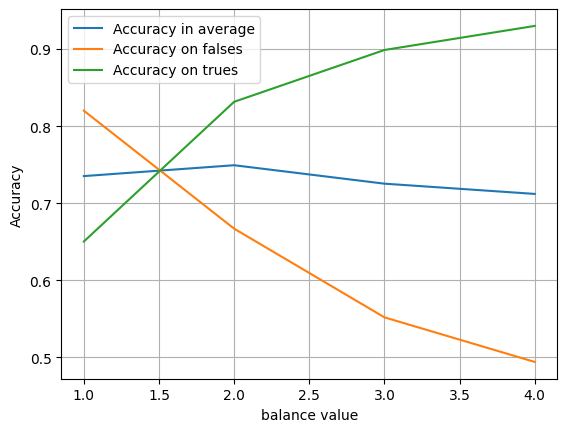
\includegraphics[width=\linewidth]{balancek5.png}
    \caption{k=5}
  \end{subfigure}%
  \hfill
  \begin{subfigure}[t]{0.33\textwidth}
    \centering
    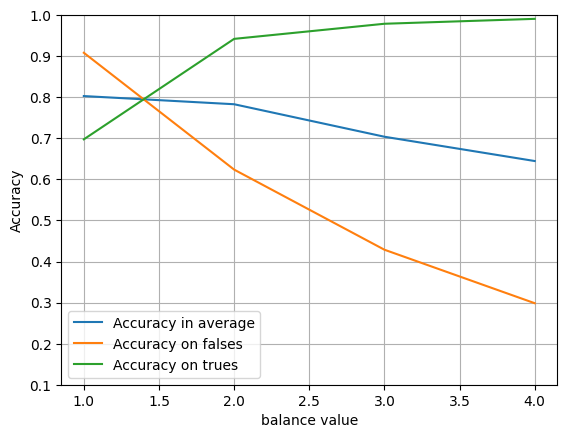
\includegraphics[width=\linewidth]{balancek50.png}
    \caption{k=50}
  \end{subfigure}
  \hfill
  \begin{subfigure}[t]{0.33\textwidth}
    \centering
    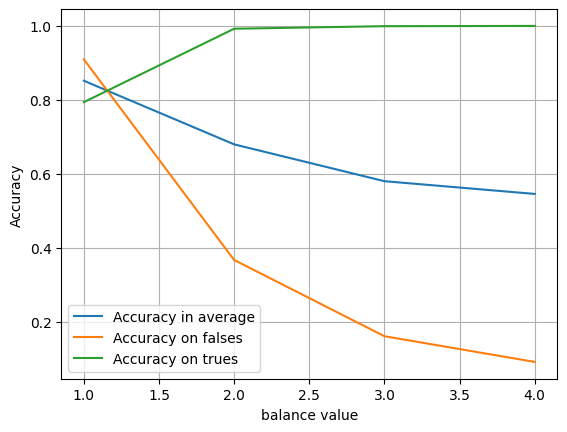
\includegraphics[width=\linewidth]{balancek500.png}
    \caption{k=500}
  \end{subfigure}
  \caption{Figure with Multiple Images}
  \label{fig:balancenk}
\end{figure}

\paragraph{On the implementation} \begin{itemize}
  \item We favor the nearer information when there is a tie.
  \item Python is not a well typed language, it is so easy to have
  ridiculous bugs.
  \item Cosine distance works much better than euclidean distance.
  \item When the data is disporpotionally labelled, we need to balance the data to ensure performance for prediction of each label.
  \item We sometime use implemented fonctions to improve
  efficacity after having understood the method and
  implemented ourselves.
\end{itemize}

\paragraph{Positive} \begin{itemize}
  \item Easy to implement
\end{itemize}

\paragraph{Negative} \begin{itemize}
  \item Supervised
  \item $\Theta(n)$ for each prediction ($n$ the size of training data), which is
  very slow when we want to use a big training data to ensure better prediction.
\end{itemize}

\subsection{Naive Bayes}

Naive Bayes is a probabilistic classification algorithm.
It is called naive because it assumes that each input variable is independent.

We are looking for: $ \max_{y}\mathbb{P}(Y =y \mid X=(x_1, ..., x_n) $

using the Naive Bayes formula: $\mathbb{P}(Y \mid X)) = \frac{\mathbb{P}(X\mid Y)\cdot \mathbb{P}(Y)}{\mathbb{P}(X)} = \frac{\mathbb{P}(Y)\prod_{i}^{}\mathbb{P}(X_i\mid Y)}{\mathbb{P}(X)}$
by independence.
where $\mathbb{P}(X\mid Y)$ is the likelihood, $\mathbb{P}(X)$ is the evidence, $\mathbb{P}(Y \mid X)$ is the posterior and $\mathbb{P}(Y)$ is the prior.


\paragraph{Advantages} \begin{itemize}
\item Even though the independence assumption is rarely true, the model is still effective
\item Handles high dimensional data well
\end{itemize}

\paragraph{Inconvenients} \begin{itemize}
\item Estimated probability is often inaccurate because of the naive assumption
\end{itemize}
\subsection{Perceptron}

\paragraph{On the implementation}
% \begin{itemize}
% \end{itemize}

\section{Testing and evalutation of models}

\paragraph{On the implementation} \begin{itemize}
  \item Ability to specify a random seed.
\end{itemize}

\section{Topological data analysis, persistent homology}

Let's introduce some terms to enable a better understood discussion.

\begin{definition}[$p$-simplex ($p\in\N$)]
  Let $V$ be some finite set (the vertices).
  A $p$-simplex $\sigma$ is the convex hull of $p+1$
  points $x_0, \ldots, x_p \in V$.
  We denote $\sigma = \conv\{x_0, \ldots, x_p\}$ a subset of $V$.
\end{definition}
\RM In practice, we simplify a topological space to its homology equivalence (thin
triangulation) without
losing the information we want (connected compoenents, holes).

\begin{definition}[Face]
  A face of $\sigma$ is $\conv(S)$ where $S\subset\{x_0,\ldots, x_p\}$
\end{definition}

\begin{definition}[Simplicial complex]
  A simplicial complex $X$ is a finite collection of simplices s.t.
  $$
  \forall \sigma\in X, \forall \tau\subset\sigma, \tau\in X
  $$
\end{definition}

\begin{definition}[Chain space]
  The vectorial space of $k$-chains of a simplicial complex $X$ over a field $\K$ is defined by:
  $$
  C_k(X) := \left\{\sum_{i=1}^{\left|X_k\right|} \alpha_i \sigma_i: \alpha_i \in \mathbb{X}, \sigma_i \in X_k\right\}
  \simeq \K^{|X_k|}
  $$
\end{definition}

\begin{definition}[$p$-chain]
  A $p$-chain is a subset of $p$-simplices in a simplicial complex $X$.
\end{definition}

\begin{definition}[Boundary operator]
  $$
  \begin{aligned}
  \partial_k: C_k(X) & \to C_{k-1}(X) \\
  \sigma=[v_0, \ldots, v_k] & \mapsto \sum_{j=0}^k(-1)^j \underbrace{[v_0,\ldots, \widehat{v}_j, \ldots, v_k]}_{\in X_{k-1}} \\
  \left(\lambda \sigma+\sigma^{\prime}\right) & \mapsto \lambda \partial_k \sigma+\partial_k \sigma^{\prime} \text{ (linear extension)}
  \end{aligned}
  $$
\end{definition}

\begin{definition}[$k$-th homology group]
  \begin{itemize}
    \item $k$-cycles : $Z_k:=\Ker(\partial_k)$
    \item $k$-boundaries : $B_k:=\Im(\partial_{k+1})$
  \end{itemize}
  The $k$-th homology group of $X$ for the field $\K$ is the following quotient
  of vector spaces:
  $$
  H_k(X):={Z_k\over B_k}
  $$
  The $k$-th Betti number $\beta_k = \mathrm{rank}(H_k)$.
\end{definition}

\begin{definition}[Filtration]
  A filtration over $T$ is a family $\F = (F_t)_{t\in T}$ of increasing topological spaces:
  $$
  \forall t, t^{\prime} \in T, t \leqslant t^{\prime} \Rightarrow F_t \subset F_{t^{\prime}}
  $$
\end{definition}

\begin{definition}[Persistence module]
  Let $\mathbb{K}$ be a given field. A persistence module over $T \subset \mathbb{R}$ is a family $\mathbb{V}=\left(V_t\right)_{t \in T}$ of $\mathbb{K}$-vector spaces endowed with linear application $v_t^{t^{\prime}}: V_t \rightarrow V_{t^{\prime}}$ such that:
  $$
  \begin{aligned}
  & \forall t \in T, v_t^t=i d \\
  & \forall t \leqslant t^{\prime} \leqslant t^{\prime \prime} \in T, v_{t^{\prime}}^{t^{\prime \prime}} \circ v_t^{t^{\prime}}=v_t^{t^{\prime \prime}}
  \end{aligned}
  $$
  (functoriality conditions)
\end{definition}

\begin{figure}[htbp]
\centering
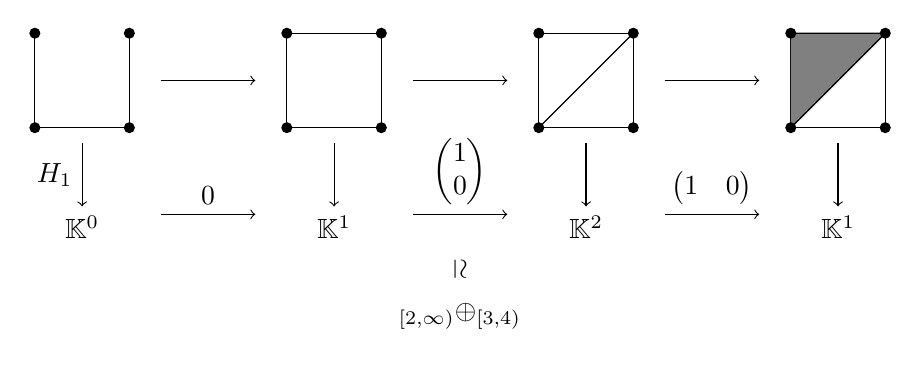
\begin{tikzpicture}[scale=0.4]

  \coordinate (v1) at (0,0);
  \coordinate (v2) at (0,3);
  \coordinate (v3) at (3,0);
  \coordinate (v4) at (3,3);
  \draw (v1) -- (v2);
  \draw (v3) -- (v4);
  \draw (v1) -- (v3);

  \coordinate (w1) at (8+0,0);
  \coordinate (w2) at (8+0,3);
  \coordinate (w3) at (8+3,0);
  \coordinate (w4) at (8+3,3);
  \draw (w1) -- (w2);
  \draw (w3) -- (w4);
  \draw (w1) -- (w3);
  \draw (w2) -- (w4);
  \draw[->] (4,1.5) -- (7,1.5);

  \coordinate (u1) at (16+0,0);
  \coordinate (u2) at (16+0,3);
  \coordinate (u3) at (16+3,0);
  \coordinate (u4) at (16+3,3);
  \draw (u1) -- (u2);
  \draw (u3) -- (u4);
  \draw (u1) -- (u3);
  \draw (u2) -- (u4);
  \draw (u1) -- (u4);
  \draw[->] (12,1.5) -- (15,1.5);

  \coordinate (uu1) at (24+0,0);
  \coordinate (uu2) at (24+0,3);
  \coordinate (uu3) at (24+3,0);
  \coordinate (uu4) at (24+3,3);
  \draw (uu1) -- (uu2);
  \draw (uu3) -- (uu4);
  \draw (uu1) -- (uu3);
  \draw (uu2) -- (uu4);
  \draw (uu1) -- (uu4);
  \filldraw[fill=gray] (uu1) -- (uu4) -- (uu2);
  \draw[->] (20,1.5) -- (23,1.5);

  \foreach \vertex in {v1,v2,v3,v4,w1,w2,w3,w4,
  u1,u2,u3,u4,
  uu1,uu2,uu3,uu4}
    \fill (\vertex) circle (5pt);

  \coordinate (d) at (1.5,-0.5);
  \draw[->] ($(v1)+(d)$) -- node[left] {$H_1$} ++(0,-2) node[below] {$\K^0$};
  \draw[->] ($(w1)+(d)$) -- ++(0,-2) node[below] {$\K^1$};
  \draw[->] ($(u1)+(d)$) -- ++(0,-2) node[below] {$\K^2$};
  \draw[->] ($(uu1)+(d)$) -- ++(0,-2) node[below] {$\K^1$};

  \draw[->] (4, -2.75) -- node[above] {$0$}++(3,0);
  \draw[->] (12,-2.75) -- node[above] {$\begin{pmatrix}1\\0 \end{pmatrix}$}++(3,0);
  \draw[->] (20,-2.75) -- node[above] {$\begin{pmatrix}1 & 0 \end{pmatrix}$}++(3,0);
  
  \node at (13.5,-4.5) {\rotatebox{270}{$\simeq$}};
  \node at (13.5,-6) {$\I_{[2, \infty)} \oplus \I_{[3, 4)}$};

\end{tikzpicture}
\end{figure}

\subsection{Essay grading}

Intuitively, a better discoursive essay should have a
richer writting structure, (a proposition should be discussed
in different angles, the last paragraph echos to the beginning)
in homology, if a good essay is a topological space, it should have
many holes (homological groups).

todo: explain more with pictures.

% \begin{figure}
% \centering
% \includegraphics[width=8cm]{persistence_diagram.png}
% \end{figure}

\paragraph{Similarity Filtration with Time Skeleton (SIFTS) \cite{Zhu_2013}}

todo: show persistence diagrams of essays of different grades.

todo: Length affects, but not much.

\printbibliography

\end{document}
